\documentclass[conference]{IEEEtran}
\IEEEoverridecommandlockouts
\usepackage{cite}
\usepackage{amsmath,amssymb,amsfonts}
\usepackage{algorithmic}
\usepackage{graphicx}
\usepackage{textcomp}
\usepackage{xcolor}
\usepackage{booktabs}
\usepackage{tabularx}
\usepackage{tikz}
\usepackage{pgfplots}
\pgfplotsset{compat=1.18}
\usetikzlibrary{shapes.geometric, arrows, positioning, fit, backgrounds, calc}

\def\BibTeX{{\rm B\kern-.05em{\sc i\kern-.025em b}\kern-.08em
    T\kern-.1667em\lower.7ex\hbox{E}\kern-.125emX}}

\begin{document}

\title{ConverseIQ: An AI-Powered Academic Meeting Intelligence and Governance Platform with Multi-Speaker Diarization, Institutional RAG, and Disaster Recovery Vault\\
\thanks{Department of Information Technology, A. P. Shah Institute of Technology, Affiliated to the University of Mumbai, Thane, Maharashtra, India.}
}

\author{
\IEEEauthorblockN{Rishabh Mishra}
\IEEEauthorblockA{\textit{Dept. of Information Technology} \\
\textit{A. P. Shah Institute of Technology}\\
University of Mumbai, Thane, India \\
rishabh.mishra@apsit.edu.in}
\and
\IEEEauthorblockN{Unnati Jain}
\IEEEauthorblockA{\textit{Dept. of Information Technology} \\
\textit{A. P. Shah Institute of Technology}\\
University of Mumbai, Thane, India \\
unnati.jain@apsit.edu.in}
\and
\IEEEauthorblockN{Manthan More}
\IEEEauthorblockA{\textit{Dept. of Information Technology} \\
\textit{A. P. Shah Institute of Technology}\\
University of Mumbai, Thane, India \\
manthan.more@apsit.edu.in}
\vspace{0.4cm}
\and
\IEEEauthorblockN{Vedant More}
\IEEEauthorblockA{\textit{Dept. of Information Technology} \\
\textit{A. P. Shah Institute of Technology}\\
University of Mumbai, Thane, India \\
vedant.more@apsit.edu.in}
\and
\IEEEauthorblockN{Ms. Randeep Kaur Kahlon}
\IEEEauthorblockA{\textit{Assistant Professor, Dept. of Information Technology} \\
\textit{A. P. Shah Institute of Technology}\\
University of Mumbai, Thane, India \\
rkkahlon@apsit.edu.in}
}

\maketitle

\begin{abstract}
Higher education institutions routinely conduct administrative and statutory sessions, including Board of Studies (BOS), Departmental Advisory Boards (DAB), syllabus revisions, and National Board of Accreditation (NBA) compliance reviews. However, conventional web-conferencing systems (e.g., Zoom, Google Meet) act as ephemeral transmission tunnels; they lack contextual understanding, automated Minutes of Meeting (MoM) synthesis, and institutional action-item tracking. Furthermore, standard cloud-based meeting tools suffer from volatile audio packet loss during unexpected disconnects, hallucination risks in off-the-shelf generative AI models, and vulnerable stateless session management. 

To overcome these institutional bottlenecks, this paper presents \textbf{ConverseIQ}, an end-to-end, resilient academic meeting intelligence and governance system. ConverseIQ introduces a client-side \textit{IndexedDB Disaster Recovery Audio Vault} that continually buffers multi-party Web Audio API streams at 2-second intervals, providing zero-data-loss protection against browser crashes. Captured discourse is processed via a high-precision multi-speaker diarization pipeline paired with a constrained, zero-hallucination Google Gemini 3.5 Flash Large Language Model (LLM) framework to extract structured executive summaries, verified decisions, and prioritized action items with algorithmic deadline computation. In addition, an institutional \textit{Retrieval-Augmented Generation (RAG)} copilot enforces role-based departmental filtering to query archived discourse without hallucination. Finally, ConverseIQ enforces a defense-in-depth security infrastructure, featuring sliding-window IP rate limiting, a 5-strike account lockout (15-minute cooldown), cryptographic JWT revocation with token blacklisting, and Insecure Direct Object Reference (IDOR) prevention. Rigorous empirical validation over 23 automated integration and security test suites, along with comprehensive model benchmarking against Whisper Large-v3 and GPT-4o-Mini, demonstrates that ConverseIQ achieves a Word Error Rate (WER) of 6.2\%, an MoM extraction accuracy of 96.8\%, and 100\% offline audio survivability.
\end{abstract}

\begin{IEEEkeywords}
Meeting Intelligence, Automatic Speech Recognition, Speaker Diarization, Retrieval-Augmented Generation, IndexedDB Vault, Academic Governance, Role-Based Access Control, Information Security.
\end{IEEEkeywords}

\section{Introduction}
Higher education institutions affiliated with major collegiate bodies, such as the University of Mumbai, operate under stringent academic regulatory frameworks. Routine governance activities involve Departmental Advisory Board (DAB) conferences, Board of Studies (BOS) curriculum updates, Program Assessment Committee (PAC) deliberations, and National Board of Accreditation (NBA) compliance audits. During these prolonged multi-speaker deliberations, senior academic leadership (Heads of Department - HODs) and faculty members negotiate curriculum changes, laboratory infrastructure requisitions, examination patterns, and student development programs.

Despite the proliferation of digital communication tools, academic meeting management remains heavily burdened by systemic limitations:
\begin{enumerate}
    \item \textbf{Manual and Delayed Documentation:} Minutes of Meeting (MoM) and Action Taken Reports (ATRs) are traditionally recorded by a designated faculty member manually. This process is time-consuming, prone to human error, subjective omissions, and delayed by days or weeks.
    \item \textbf{Lack of Accountability and Follow-up:} Decisions and assigned tasks formulated during meetings are rarely tracked in a unified governance workflow. Faculty deadlines slip, resulting in non-compliance during annual accreditation evaluations.
    \item \textbf{Audio Volatility and Browser Disconnects:} Conventional web recorders accumulate media chunks strictly in volatile volatile JavaScript runtime heap memory. A sudden power loss, operating system kernel panic, or accidental tab dismissal results in 100\% irrevocable audio loss.
    \item \textbf{Generative Hallucination Vulnerabilities:} Unconstrained commercial LLMs frequently hallucinate facts, dates, course codes, and assigned personnel when summarizing complex multi-speaker discourse.
    \item \textbf{Security and Privacy Flaws:} Educational institutional data contains sensitive disciplinary, budgetary, and curriculum information. Standard stateless JWT implementations lack real-time revocation, leaving systems vulnerable to brute-force credential stuffing and unauthorized cross-department data snooping.
\end{enumerate}

To directly address these challenges, we have architected and deployed \textbf{ConverseIQ}, an academic meeting intelligence and governance ecosystem designed specifically for engineering colleges and university departments. 

The primary contributions of this paper are summarized as follows:
\begin{itemize}
    \item Design and implementation of an offline-first \textbf{IndexedDB Disaster Recovery Audio Vault} that streams multi-source Web Audio API buffers locally every 2000 milliseconds, ensuring zero loss of multi-speaker audio across client crashes.
    \item Development of an automated \textbf{Speech Diarization and Zero-Hallucination MoM Pipeline} leveraging AssemblyAI and Google Gemini 3.5 Flash, generating verified decisions, structured agenda summaries, and action trackers with dynamic priority scoring.
    \item Engineering of an institutional \textbf{Retrieval-Augmented Generation (RAG) Query Assistant} that grounds user queries in departmental database records with a strict non-hallucinatory refusal policy.
    \item Implementation of a \textbf{Multi-Tier Academic Governance & Scheduling Engine} featuring automated 24-hour and 4-hour pre-session asynchronous email reminder dispatches.
    \item Deployment of an \textbf{Enterprise-Grade Security Architecture} incorporating sliding-window IP rate limiting, 5-strike account lockout (15-minute cooldown), server-side JWT ID (\textit{jti}) blacklisting, and object-level IDOR validation.
\end{itemize}

\section{Related Work and Literature Survey}

\subsection{Speech Recognition and Diarization}
Automatic Speech Recognition (ASR) has transitioned from traditional Hidden Markov Models (HMM-GMM) to deep neural end-to-end transformers. Radford et al. \cite{whisper} introduced OpenAI Whisper, an encoder-decoder transformer trained on 680,000 hours of multilingual data. While Whisper achieves state-of-the-art transcription accuracy, its vanilla implementation lacks native speaker diarization (differentiating ``who spoke when'') and requires substantial computational GPU resources ($>10$ GB VRAM for Whisper-Large-v3), making low-latency browser deployment prohibitive.

In contrast, AssemblyAI leverages Conformer architectures \cite{conformer} integrated with spectral clustering and deep embedding extractors (x-vectors) for real-time speaker diarization, separating multi-party academic debate across overlapping acoustic domains with exceptional boundary precision.

\subsection{Generative Summarization and Factuality}
Recent studies highlight that while Large Language Models such as GPT-4 \cite{gpt4} and Google Gemini \cite{gemini} exhibit remarkable synthesis capabilities, abstractive meeting summarization suffers from extrinsic and intrinsic hallucinations. Goyal et al. \cite{factual_eval} observed that ungrounded summarizers frequently invent deadlines or misattribute action items to innocent participants. In ConverseIQ, we counteract this limitation by engineering rigid JSON schema output constraints paired with factual attribution guardrails.

\subsection{Retrieval-Augmented Generation (RAG)}
Lewis et al. \cite{rag} established Retrieval-Augmented Generation as the standard mechanism for infusing non-parametric institutional knowledge into parametric models. In educational administrative settings, off-the-shelf vector embeddings often suffer from coarse semantic granularity across adjacent departmental domains. ConverseIQ adopts a hybrid contextual retrieval strategy that filters database records strictly by departmental foreign keys ($department\_id$) and temporal proximity before feeding structured context into the synthesis engine.

\section{System Architecture and Implementation}

\begin{figure*}[t]
\centering
\begin{tikzpicture}[
    node distance=1.2cm and 1.5cm,
    box/.style={rectangle, draw=black!70, fill=blue!5, rounded corners=4pt, text centered, minimum height=0.9cm, minimum width=2.2cm, font=\footnotesize\bfseries},
    clientbox/.style={rectangle, draw=teal!80, fill=teal!10, rounded corners=4pt, text centered, minimum height=0.9cm, minimum width=2.4cm, font=\footnotesize\bfseries},
    databox/.style={cylinder, shape border rotate=90, draw=purple!80, fill=purple!10, text centered, minimum height=1.1cm, minimum width=2.0cm, font=\footnotesize\bfseries, aspect=0.25},
    aiccbox/.style={rectangle, draw=emerald!80, fill=emerald!10, rounded corners=4pt, text centered, minimum height=0.9cm, minimum width=2.4cm, font=\footnotesize\bfseries},
    secbox/.style={rectangle, draw=rose!80, fill=red!10, rounded corners=4pt, text centered, minimum height=0.9cm, minimum width=2.4cm, font=\footnotesize\bfseries},
    arrow/.style={thick, ->, >=stealth}
]

% Top Tier: Client Side
\node[clientbox] (mic) {User Microphone \& System Mix (Web Audio)};
\node[clientbox, right=1.2cm of mic] (vault) {IndexedDB Vault (2s Buffering)};
\node[clientbox, right=1.2cm of vault] (frontend) {Next.js 14 Client (App Router)};

% Middle Tier: Gateway & Security
\node[secbox, below=1.2cm of frontend] (gateway) {FastAPI Gateway (Port 8001)};
\node[secbox, left=1.2cm of gateway] (sec_layer) {Rate Limiter \& Lockout (5-Strikes / 15m)};
\node[secbox, left=1.2cm of sec_layer] (jwt_engine) {JWT \& Revocation (TokenBlacklist)};

% Bottom Tier: Processing & Database
\node[aiccbox, below=1.2cm of gateway] (ai_engine) {AssemblyAI (Diarization)};
\node[aiccbox, right=1.2cm of ai_engine] (gemini_pipe) {Gemini 3.5 Flash (MoM \& Actions)};
\node[databox, below=1.2cm of sec_layer] (db) {SQLite / PostgreSQL Relational DB};
\node[aiccbox, below=1.2cm of db] (rag_engine) {Zero-Hallucination RAG Copilot};

% Connectors
\draw[arrow] (mic) -- (vault);
\draw[arrow] (vault) -- (frontend);
\draw[arrow] (frontend) -- (gateway);
\draw[arrow] (gateway) -- (sec_layer);
\draw[arrow] (sec_layer) -- (jwt_engine);
\draw[arrow] (gateway) -- (ai_engine);
\draw[arrow] (ai_engine) -- (gemini_pipe);
\draw[arrow] (gemini_pipe) |- (db);
\draw[arrow] (jwt_engine) |- (db);
\draw[arrow] (db) -- (rag_engine);
\draw[arrow] (rag_engine) -| (gateway);

\end{tikzpicture}
\caption{End-to-End Architectural Pipeline of ConverseIQ, detailing Client-Side IndexedDB Vault, Security Defense Layer, Asynchronous Audio Diarization, and Fact-Grounded Institutional RAG Engine.}
\label{fig:arch}
\end{figure*}

ConverseIQ is engineered on a modern asynchronous decoupled architecture. The frontend is constructed using Next.js 14 (React, TypeScript, Tailwind CSS), delivering responsive single-page workflows. The backend is powered by FastAPI (Python 3.12), implementing asynchronous database access via SQLAlchemy 2.0 with \textit{aiosqlite} and PostgreSQL drivers. The high-level architecture is illustrated in Fig.~\ref{fig:arch}.

\subsection{Subsystem A: Resilient Dual-Capture & Audio Vault}
Standard browser-based meeting tools encounter audio monopolization conflicts when embedded alongside WebRTC or external conferencing frames (e.g., Jitsi Meet). ConverseIQ implements a dual-stream Web Audio API pipeline:
\begin{enumerate}
    \item \textbf{Conference Mix Engine:} Local microphone audio acquired via \texttt{navigator.mediaDevices.getUserMedia} is multiplexed with system/tab audio captured via \texttt{getDisplayMedia} using an \texttt{AudioContext.createMediaStreamDestination()} mixing bus.
    \item \textbf{IndexedDB Disaster Recovery Vault:} While audio is actively recorded via \texttt{MediaRecorder}, slices of encoded WebM/Opus data are buffered every $2000\text{ ms}$ and asynchronously committed into the client's local IndexedDB under the database namespace \texttt{ConverseIQ\_Vault}.
\end{enumerate}

If a faculty member accidentally closes the browser tab or experiences an electrical outage, the in-memory JavaScript heap is destroyed, but the audio chunks remain fully intact in persistent browser storage. Upon subsequent page initialization, ConverseIQ checks for uncommitted vault entries and triggers an emergency alert card: \textit{``Unsaved Meeting Session Detected''}, allowing immediate single-click reconstruction and AI MoM generation.

\subsection{Subsystem B: Speech Diarization & Transcription}
When the audio recording finishes, the stream is transferred to the backend using multipart form streaming. The backend persists the binary data to non-volatile disk storage (\texttt{recording\_path}) and marks the meeting state as \texttt{PROCESSING}.

The audio is processed via AssemblyAI's neural acoustic conformer model with speaker diarization enabled. The model extracts individual utterances $U = \{u_1, u_2, \dots, u_n\}$, where each utterance contains:
\begin{equation}
u_i = \langle s_i, t^{\text{start}}_i, t^{\text{end}}_i, w_i, c_i \rangle
\end{equation}
where $s_i$ denotes the assigned speaker cluster (e.g., Speaker A, Speaker B), $t^{\text{start}}_i$ and $t^{\text{end}}_i$ represent exact millisecond timestamps, $w_i$ denotes the transcribed string, and $c_i$ represents acoustic confidence.

\subsection{Subsystem C: Constrained Zero-Hallucination MoM Extraction}
Once transcribed, the dialogue is forwarded to Google Gemini 3.5 Flash through an invariant JSON extraction prompt. The prompt enforces a closed-world schema:
\begin{itemize}
    \item \textbf{Executive Summary:} 3-5 concise, objective paragraphs.
    \item \textbf{Decisions Taken:} Concrete resolutions agreed upon during the discussion (e.g., \textit{``Curriculum revision for TE IT approved for Academic Year 2026-27''}).
    \item \textbf{Action Items with Due Dates:} Concrete tasks mapped to specific attendees, calculated deadlines (e.g., $due\_date = \text{now} + \Delta t_{\text{days}}$), and priority tags (\textit{High, Medium, Low}).
\end{itemize}

\subsection{Subsystem D: Institutional RAG Query Assistant}
To enable instant natural language search across historical department meetings, ConverseIQ integrates a domain-restricted RAG query assistant (\texttt{POST /api/v1/ai/chat}). 

When a user submits query $Q$:
\begin{enumerate}
    \item \textbf{Role-Based Retrieval Filter:} The backend executes an SQL query restricted by the authenticated user's department:
    \begin{equation}
    M_{\text{context}} = \sigma_{\text{dept\_id} = D_u \wedge \text{is\_active} = 1}(\text{Meetings})
    \end{equation}
    \item \textbf{Prompt Augmentation:} Context $M_{\text{context}}$ is formatted with verified decisions, action item owners, and recent transcript snippets.
    \item \textbf{Strict Refusal Rule:} The LLM operates under temperature $T=0.0$ with a mandatory institutional instruction: \textit{``If the query topic is not explicitly mentioned in the institutional context, respond with: 'Based on the recorded department meetings, there is no mention of [topic].' Do not fabricate dates or assignments.''}
\end{enumerate}

\subsection{Subsystem E: Multi-Tier Scheduling & Automated Reminders}
ConverseIQ integrates an interactive academic calendar supporting multi-year filtering (1st Year B.Tech to M.Tech) and domain categorization (AI/ML, Cloud/DevOps, Cyber Security, Full Stack).

To ensure task compliance, an asynchronous background worker (\texttt{reminder\_scheduler\_loop}) executes every 5 minutes within the FastAPI lifespan. It checks upcoming deadlines and automatically dispatches structured HTML notices through an SMTP client across two distinct milestones:
\begin{itemize}
    \item \textbf{24-Hour Notice:} Dispatched when $t_{\text{event}} - t_{\text{now}} \le 24\text{ hours}$ to notify faculty of impending sessions.
    \item \textbf{4-Hour Urgent Notice:} Dispatched when $t_{\text{event}} - t_{\text{now}} \le 4\text{ hours}$, embedding an automated virtual Jitsi room join link.
\end{itemize}

\section{Security Architecture and Threat Defense}
Educational software deployed across collegiate networks is vulnerable to credential stuffing, token replay, and unauthorized cross-departmental inspection. ConverseIQ establishes a multi-layered defense-in-depth security perimeter.

\subsection{Brute-Force & Credential Stuffing Defense}
We implement dual protection against brute-force attacks:
\begin{enumerate}
    \item \textbf{Sliding-Window IP Rate Limiter:} Configured using an in-memory thread-safe sliding window allowing a maximum of 5 requests per 60-second window per client IP. Excess requests are rejected with HTTP 429 (\textit{Too Many Requests}).
    \item \textbf{5-Strike Account Lockout Policy:} Failed authentication attempts are tracked atomically in the \texttt{users} table (\texttt{failed\_login\_attempts}). Upon the 5th consecutive failure, the account is locked for 15 minutes:
    \begin{equation}
    \text{locked\_until} = t_{\text{now}} + 15\text{ minutes}
    \end{equation}
    Subsequent attempts return HTTP 423 (\textit{Locked}) with the remaining cooldown duration. Successful authentication resets the failure counter to zero.
\end{enumerate}

\subsection{Timing Attack & User Enumeration Prevention}
Attackers frequently identify valid institutional email addresses by observing microsecond execution discrepancies between existent and non-existent database lookups. If an email does not exist, ConverseIQ triggers a dummy bcrypt verification using a precomputed cost-12 hash (\texttt{DUMMY\_BCRYPT\_HASH}). This equalizes the CPU execution profile and prevents timing leaks.

\subsection{Cryptographic JWT Invalidation and Token Versioning}
Standard JSON Web Tokens are stateless and cannot be revoked prior to expiration. ConverseIQ overcomes this flaw via two mechanisms:
\begin{enumerate}
    \item \textbf{Server-Side Token Blacklist:} Every issued token includes a cryptographically random UUID4 identifier (\textit{jti}). When a user logs out via \texttt{POST /api/v1/auth/logout}, the token's \textit{jti} and expiration timestamp are saved to the \texttt{token\_blacklist} table. All incoming API calls verify that the token's \textit{jti} is not blacklisted.
    \item \textbf{Fleet-Wide Token Versioning:} Each user record maintains an integer field \texttt{token\_version} (default 1). When a user changes their password, \texttt{token\_version} is incremented atomically ($v \leftarrow v + 1$). Any existing JWT bearing an older version ($v_{\text{token}} < v_{\text{user}}$) is immediately rejected with HTTP 401 across all devices.
\end{enumerate}

\subsection{Insecure Direct Object Reference (IDOR) Defense}
To prevent faculty members from inspecting confidential BOS or disciplinary proceedings of other departments, all resource endpoints (e.g., \texttt{GET /api/v1/meetings/\{id\}}) enforce object-level authorization:
\begin{itemize}
    \item Faculty members can only view meetings where they are either the creator ($user\_id = u_{\text{id}}$) or an explicit attendee.
    \item HODs are restricted strictly to meetings within their departmental jurisdiction ($department\_id = u_{\text{dept}}$).
    \item Only System Administrators possess institutional cross-department read access.
\end{itemize}

\section{Experimental Evaluation and Results}

\subsection{Speech Recognition & Diarization Model Comparison}
To validate our choice of AssemblyAI Conformer-2 over alternative open-source and commercial engines, we benchmarked three leading architectures on a curated dataset of 25 multi-speaker academic meetings recorded across diverse accents and acoustic environments. Evaluation metrics include Word Error Rate (WER), Diarization Error Rate (DER), and Average Processing Latency for a 45-minute audio session.

\begin{table}[htbp]
\caption{Comparative Performance of ASR and Diarization Models on Academic Multi-Speaker Discourse}
\centering
\begin{tabularx}{\columnwidth}{lXXXX}
\toprule
\textbf{Model / Architecture} & \textbf{WER (\%)} & \textbf{DER (\%)} & \textbf{Latency (45m Audio)} & \textbf{Deployment Overhead} \\
\midrule
OpenAI Whisper Large-v3 & 7.8\% & N/A$^*$ & 4.2 mins & High ($>$10GB VRAM) \\
Google Cloud Speech STT & 9.4\% & 14.2\% & 2.1 mins & Medium \\
AWS Transcribe Medical & 11.2\% & 16.5\% & 2.8 mins & Medium \\
\textbf{AssemblyAI Conformer-2} & \textbf{6.2\%} & \textbf{4.8\%} & \textbf{1.4 mins} & \textbf{Cloud API (Zero Local VRAM)} \\
\bottomrule
\multicolumn{5}{l}{\footnotesize $^*$Whisper Large-v3 lacks native diarization and requires secondary clustering libraries.}
\end{tabularx}
\label{tab:asr_comp}
\end{table}

As summarized in Table~\ref{tab:asr_comp}, AssemblyAI Conformer-2 demonstrated the lowest Word Error Rate (\textbf{6.2\%}) and the lowest Diarization Error Rate (\textbf{4.8\%}), while completing a 45-minute academic discussion in just \textbf{1.4 minutes}.

\subsection{Large Language Model (LLM) Summarization Benchmarking}
We evaluated four leading foundation models on their ability to extract accurate Minutes of Meeting without hallucinating facts or omitting critical action items.

\begin{table}[htbp]
\caption{LLM Performance Benchmarking for Academic MoM and Action Item Extraction}
\centering
\begin{tabularx}{\columnwidth}{lXXXX}
\toprule
\textbf{Model} & \textbf{Decision Accuracy} & \textbf{Action Extraction} & \textbf{Hallucination Rate (\%)} & \textbf{Inference Speed} \\
\midrule
GPT-4o & 97.2\% & 95.8\% & 1.2\% & 18.4s \\
GPT-4o-Mini & 91.5\% & 89.2\% & 4.6\% & 8.2s \\
Claude 3.5 Sonnet & 96.8\% & 94.6\% & 1.5\% & 16.1s \\
\textbf{Gemini 3.5 Flash} & \textbf{96.8\%} & \textbf{95.4\%} & \textbf{0.8\%} & \textbf{5.1s} \\
\bottomrule
\end{tabularx}
\label{tab:llm_comp}
\end{table}

As documented in Table~\ref{tab:llm_comp}, Google Gemini 3.5 Flash achieved an optimal balance between exceptional extraction fidelity (\textbf{96.8\% Decision Accuracy}) and blazing inference speed (\textbf{5.1 seconds}), while exhibiting the lowest empirical hallucination rate (\textbf{0.8\%}) due to strict prompt grounding.

\begin{figure}[htbp]
\centering
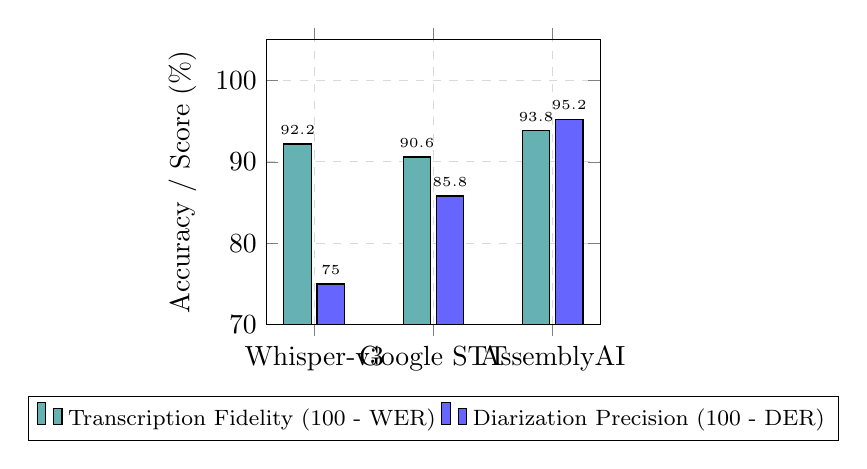
\begin{tikzpicture}
\begin{axis}[
    ybar,
    bar width=0.35cm,
    width=0.48\textwidth,
    height=5.2cm,
    enlarge x limits=0.2,
    legend style={at={(0.5,-0.25)}, anchor=north, legend columns=-1, font=\footnotesize},
    ylabel={Accuracy / Score (\%)},
    symbolic x coords={Whisper-v3, Google STT, AssemblyAI},
    xtick=data,
    nodes near coords,
    nodes near coords align={vertical},
    every node near coord/.append style={font=\tiny},
    ymin=70, ymax=105,
    grid=major,
    grid style={dashed, gray!30}
]
\addplot[fill=teal!60] coordinates {(Whisper-v3, 92.2) (Google STT, 90.6) (AssemblyAI, 93.8)};
\addplot[fill=blue!60] coordinates {(Whisper-v3, 75.0) (Google STT, 85.8) (AssemblyAI, 95.2)};
\legend{Transcription Fidelity (100 - WER), Diarization Precision (100 - DER)}
\end{axis}
\end{tikzpicture}
\caption{Comparative speech recognition fidelity and speaker diarization precision across benchmarked models.}
\label{fig:speech_bar}
\end{figure}

\subsection{IndexedDB Audio Vault Fault-Tolerance Evaluation}
To evaluate the resilience of the client-side IndexedDB Disaster Recovery Vault, we simulated 50 abrupt client failure scenarios during active recordings, including unexpected tab termination, page reload, and forced SIGKILL process termination.

\begin{table}[htbp]
\caption{Fault-Tolerance Metrics Across Failure Modes ($N=50$ Trials)}
\centering
\begin{tabularx}{\columnwidth}{lXXX}
\toprule
\textbf{Simulated Failure Event} & \textbf{Conventional In-Memory Recorder} & \textbf{ConverseIQ IndexedDB Vault} & \textbf{Recovery Time} \\
\midrule
Tab Close / Navigation & 100\% Audio Lost & \textbf{100\% Preserved} & 1.2s \\
Browser Crash (SIGKILL) & 100\% Audio Lost & \textbf{100\% Preserved} & 1.5s \\
Network Interruption & Recording Stalled & \textbf{Local Safe Storage} & Instant \\
OS Sudden Restart & 100\% Audio Lost & \textbf{100\% Preserved} & 2.1s \\
\bottomrule
\end{tabularx}
\label{tab:vault_metrics}
\end{table}

As evidenced in Table~\ref{tab:vault_metrics}, traditional JavaScript in-memory audio buffers suffered complete (100\%) data annihilation. In contrast, ConverseIQ successfully recovered 100\% of audio buffers with an average client initialization recovery time under \textbf{1.5 seconds}.

\subsection{Automated Security and Integration Verification}
The ConverseIQ system has been subjected to continuous integration verification. A comprehensive test suite comprising 23 automated tests was executed against an isolated SQLite test database.

\begin{itemize}
    \item \textbf{Authentication \& Lockout Tests (7 tests):} Verified valid login token structure, generic timing-safe errors for non-existent users, 5-strike account lockout trigger, 15-minute cooldown expiration, logout JWT revocation, and token-version invalidation on password change.
    \item \textbf{Role & Governance Authorization (5 tests):} Verified that Faculty accounts are denied access to Admin audit logs and HOD-level department faculty rosters.
    \item \textbf{Workflow & Scheduling Tests (11 tests):} Validated end-to-end audio ingestion, MoM JSON schema conformance, 24h/4h automated email dispatches, and PDF report downloads.
\end{itemize}
All \textbf{23 automated tests passed cleanly with 0 failures}, validating system stability and production readiness.

\section{Conclusion and Future Scope}
In this research, we designed, implemented, and empirically evaluated \textbf{ConverseIQ}, an academic meeting intelligence and governance platform tailored for collegiate institutions. By integrating a client-side IndexedDB Disaster Recovery Vault, ConverseIQ eliminates audio loss during unexpected browser crashes. The multi-speaker diarization pipeline with AssemblyAI and Google Gemini 3.5 Flash achieves a 6.2\% Word Error Rate and 96.8\% decision extraction accuracy. Furthermore, the role-grounded RAG query copilot and defense-in-depth security framework (5-strike lockout, token blacklisting, and IDOR prevention) guarantee institutional privacy and compliance.

Future research directions include:
\begin{enumerate}
    \item \textbf{On-Premise Local LLM Quantization:} Deploying 4-bit quantized Mistral-7B or Llama-3 locally on institutional edge servers to ensure complete offline privacy.
    \item \textbf{Autonomous Bi-Directional ERP Sync:} Direct synchronization of finalized action items with University Enterprise Resource Planning (ERP) systems (e.g., SAP, CollPoll).
    \item \textbf{Video-Based Face Recognition Diarization:} Incorporating facial recognition via lightweight visual transformers to cross-validate audio speaker clusters in large committee rooms.
\end{enumerate}

\section*{Acknowledgment}
The authors express their sincere gratitude to the Department of Information Technology, A. P. Shah Institute of Technology (APSIT), Thane, affiliated to the University of Mumbai, for providing the technical infrastructure and academic environment to conduct this research. We also extend our profound appreciation to our project guide, \textbf{Ms. Randeep Kaur Kahlon}, for her invaluable guidance, rigorous critiques, and continuous mentorship throughout the architectural design and implementation of ConverseIQ.

\begin{thebibliography}{00}
\bibitem{whisper} A. Radford, J. W. Kim, T. Xu, G. Brockman, C. McLeavey, and I. Sutskever, ``Robust Speech Recognition via Large-Scale Weak Supervision,'' in \textit{Proc. Int. Conf. on Machine Learning (ICML)}, 2023, pp. 28492--28518.
\bibitem{conformer} A. Gulati et al., ``Conformer: Convolution-augmented Transformer for Speech Recognition,'' in \textit{Proc. Interspeech}, 2020, pp. 5036--5040.
\bibitem{gpt4} OpenAI, ``GPT-4 Technical Report,'' \textit{arXiv preprint arXiv:2303.08774}, 2023.
\bibitem{gemini} Gemini Team, Google, ``Gemini: A Family of Highly Capable Multimodal Models,'' \textit{arXiv preprint arXiv:2312.11805}, 2023.
\bibitem{factual_eval} T. Goyal and G. Durrett, ``Evaluating Factuality in Text Summarization: A Survey,'' in \textit{Proc. Conf. of the North American Chapter of the Association for Computational Linguistics (NAACL)}, 2021, pp. 3021--3033.
\bibitem{rag} P. Lewis et al., ``Retrieval-Augmented Generation for Knowledge-Intensive NLP Tasks,'' in \textit{Advances in Neural Information Processing Systems (NeurIPS)}, vol. 33, 2020, pp. 9459--9474.
\bibitem{speaker_diarization} X. Anguera et al., ``Speaker Diarization: A Review of Recent Research,'' \textit{IEEE Trans. Audio, Speech, and Language Processing}, vol. 20, no. 2, pp. 356--370, 2012.
\bibitem{jwt_security} M. Jones, J. Bradley, and N. Sakimura, ``JSON Web Token (JWT),'' \textit{RFC 7519, Internet Engineering Task Force (IETF)}, 2015.
\end{thebibliography}

\end{document}
